\documentclass[a4paper,11pt,parskip=half,toc=listof,bibliography=totoc]{scrartcl}

% ------------------------------------------------------------------
% Pakete
% ------------------------------------------------------------------
\usepackage[utf8]{inputenc}
\usepackage[T1]{fontenc}
\usepackage[ngerman]{babel}
\usepackage{lmodern}
\usepackage{microtype}
\usepackage[a4paper,left=25mm,right=25mm,top=25mm,bottom=25mm]{geometry}
\usepackage{amsmath,amssymb}
\usepackage{graphicx}
\usepackage{booktabs}
\usepackage{tabularx}
\usepackage{float}
\usepackage[font=small,labelfont=bf]{caption}
\usepackage[locale=DE,per-mode=symbol,exponent-product=\cdot]{siunitx}
\usepackage{xcolor}
\usepackage{listings}
\usepackage{tikz}
\usetikzlibrary{patterns,arrows.meta}
\usepackage[hidelinks]{hyperref}

\graphicspath{{abbildungen/}}

% automatisch erzeugte Kennwerte aus MATLAB
\newcommand{\AnteilUeber}{\num{29}}
\newcommand{\AliasFaktor}{\num{1.5}}

\newcommand{\KraftMittel}{\num{0.00071}}
\newcommand{\KraftEff}{\num{2.02}}
\newcommand{\KraftAmplitude}{\num{2.86}}


\lstset{
  language=Matlab,
  basicstyle=\ttfamily\scriptsize,
  keywordstyle=\color{blue!70!black},
  commentstyle=\color{green!40!black},
  stringstyle=\color{red!60!black},
  numbers=left, numberstyle=\tiny\color{gray},
  breaklines=true, frame=single, rulecolor=\color{gray!50},
  showstringspaces=false, tabsize=4,
  literate={ä}{{\"a}}1 {ö}{{\"o}}1 {ü}{{\"u}}1 {ß}{{\ss}}1
           {Ä}{{\"A}}1 {Ö}{{\"O}}1 {Ü}{{\"U}}1
}

\newcommand{\Sx}{S_{x}}
\newcommand{\Sxx}{S_{xx}}
\newcommand{\Gxx}{G_{xx}}
\makeatletter
\newcommand{\tabinput}[1]{\@@input tabellen/#1.tex }
\makeatother
\newcommand{\abb}[1]{Abb.~\ref{#1}}
\newcommand{\tab}[1]{Tab.~\ref{#1}}

% ------------------------------------------------------------------
\begin{document}

\begin{titlepage}
  \centering
  {\large Hochschule München -- Fakultät 03\\
  Labor für Schwingungstechnik und Maschinendynamik\par}
  \vspace{3cm}
  {\Huge\bfseries Schwingungsanalyse\par}
  \vspace{0.6cm}
  {\Large Versuchsbericht MTP/VTP\par}
  \vspace{0.4cm}
  {\large Einfluss von Abtastrate, Fensterfunktion, Frequenzauflösung,\\
  Spektraldarstellung und Sensorposition auf die Signalanalyse\par}
  \vspace{3cm}
  \begin{tabular}{ll}
    \toprule
    Name & Gruppe \\
    \midrule
    Marc Hoheisel    & LRB7  \\
    Leon Nothhelfer  & LRB5  \\
    Jonas Heiermann  & LRB5P \\
    \bottomrule
  \end{tabular}
  \vfill
  \begin{tabular}{ll}
    Versuchsdatum: & 16.11.2026 \\
    Messplatz:     & Platz 1, Schwingungsanalyse am Balken \\
    Betreuer:      & Prof.\ Dr.\ Bastian Esefeld \\
    Abgabe:        & \today
  \end{tabular}
\end{titlepage}

\tableofcontents
\clearpage

% ==================================================================
\section{Einleitung und Aufgabenstellung}
% ==================================================================
Ziel des Versuchs ist das Kennenlernen der Fourier-basierten Signalanalyse
von Schwingungsmessungen und ihrer Zielkonflikte. Dazu wurden an einem
schwingungsfähigen Balken Beschleunigungs- und Kraftsignale mit einer
MATLAB-App erfasst und anschließend in MATLAB ausgewertet. Anhand der
erfassten Daten soll der Einfluss
\begin{enumerate}
  \item der Abtastrate,
  \item der Fensterfunktion,
  \item der Frequenzauflösung,
  \item der Spektraldarstellung ($\Sx$, $\Sxx$, $\Gxx$) und
  \item der Sensorposition auf der Struktur
\end{enumerate}
ermittelt und mittels Erklärungen und Darstellungen belegt werden. Grundlage
ist Kapitel~14.4 \glqq Signalanalyse im Frequenzbereich\grqq{} aus
\cite{kuttner} sowie die Versuchsunterlage \cite{esefeld}.

% ==================================================================
\section{Theoretische Grundlagen}
% ==================================================================

\subsection{Digitalisierung, Abtasttheorem und Aliasing}
Ein analoges (zeit- und wertkontinuierliches) Sensorsignal wird in der
Messkette verstärkt, durch ein analoges Tiefpassfilter bandbegrenzt, von
einer Sample-\&-Hold-Schaltung zeitdiskret abgetastet und vom A/D-Wandler
wertdiskret quantisiert. Nach dem Abtasttheorem lässt sich ein Signal nur
dann ohne Informationsverlust rekonstruieren, wenn die Abtastrate $f_s$
mindestens doppelt so groß ist wie die höchste im Signal enthaltene Frequenz:
\begin{equation}
  f_s > 2\,f_{\max} \qquad\Leftrightarrow\qquad f_{\max} < f_N = \frac{f_s}{2}.
\end{equation}
Anteile oberhalb der Nyquist-Frequenz $f_N$ werden in den Bereich
$0\ldots f_N$ gespiegelt (\emph{Aliasing}); eine Frequenz $f$ erscheint bei
\begin{equation}
  f_\text{alias} = \left| f - k\,f_s \right|, \qquad k \in \mathbb{N}
  \text{ so, dass } 0 \le f_\text{alias} \le f_N .
  \label{eq:alias}
\end{equation}
Gespiegelte Anteile sind im digitalen Signal nicht mehr von echten
Signalanteilen unterscheidbar. Deshalb muss \emph{vor} der Abtastung ein
analoges Anti-Aliasing-Tiefpassfilter (AA-Filter) eingesetzt werden. Wegen
dessen endlicher Flankensteilheit ist der Bereich knapp unterhalb von $f_N$
unbrauchbar; nutzbar ist typischerweise $f_{\max}\approx f_s/2{,}56$.
Bei impulsartigen Signalen sind deutlich höhere Abtastraten erforderlich,
da sonst Impulshöhe und -dauer falsch erfasst werden \cite{esefeld}.

\subsection{Diskrete Fouriertransformation}
Die diskrete Fouriertransformation (DFT) bildet einen Block von $N$
Abtastwerten $x(k)$ auf $N$ komplexe Spektralwerte ab:
\begin{equation}
  X(n) = \sum_{k=0}^{N-1} x(k)\, \mathrm{e}^{-\mathrm{j}2\pi kn/N},
  \qquad n = 0,\ldots,N-1 .
\end{equation}
Die \emph{FFT} (Fast Fourier Transform) ist kein anderes Ergebnis, sondern
ein effizienter Algorithmus zur Berechnung der DFT. Durch rekursive Zerlegung
(klassisch für $N=2^m$) sinkt der Rechenaufwand von $\mathcal{O}(N^2)$ auf
$\mathcal{O}(N\log_2 N)$.

Zwischen Blocklänge $T$, Abtastrate $f_s$, Linienzahl $N$ und
Frequenzauflösung $\Delta f$ gilt
\begin{equation}
  T = N\,\Delta t = \frac{N}{f_s}, \qquad
  \Delta f = \frac{1}{T} = \frac{f_s}{N}
  \qquad\Rightarrow\qquad T\cdot\Delta f = 1 .
  \label{eq:unschaerfe}
\end{equation}
Eine feine Frequenzauflösung erfordert also eine lange Blockdauer und damit
eine schlechte Zeitauflösung (Unschärferelation der Signalanalyse). Die
\emph{essentielle Annahme} der Fouriertransformation ist, dass sich das Signal
aus (phasenverschobenen) Sinusschwingungen zusammensetzt und dass der
analysierte Block eine Periode eines periodisch fortgesetzten, stationären
Signals darstellt. Ist das Signal im Block nicht periodisch, entstehen an den
Blockgrenzen Sprünge, die zum \emph{Leckeffekt} (Leakage) führen.

\subsection{Fensterfunktionen}
Durch Multiplikation des Blocks mit einer Fensterfunktion $w(k)$, die an den
Blockrändern gegen null geht, wird das Signal in einen stetigen Verlauf
gezwungen. Das Fenster verringert die Amplitude systematisch; dies wird mit
dem Fenstermittelwert $F_M$ korrigiert. Gleichzeitig verbreitert es die
effektive Bandbreite $B_\text{eff}$ einer Spektrallinie:
\begin{equation}
  F_M = \frac{1}{N}\sum_{k=0}^{N-1} w(k), \qquad
  P_M = \frac{1}{N}\sum_{k=0}^{N-1} w^2(k), \qquad
  B_\text{eff} = \frac{P_M}{T\,F_M^2} .
\end{equation}
Für das Rechteckfenster gilt $F_M = P_M = 1$ und $B_\text{eff}=\Delta f$.
Das Hanning-Fenster ist der Standard für allgemeine Analysen, das
Flattop-Fenster liefert die genauesten Amplituden periodischer Signale.

\subsection{Spektraldarstellungen}
Mit dem Spektrum $S(f)$ eines (gefensterten) Blocks werden folgende
einseitigen Darstellungen unterschieden \cite{esefeld}:
\begin{align}
  \text{Betragsspektrum:}\quad & \Sx(f) = \frac{2\,|S(f)|}{N\,F_M}
     && \text{Einheit: EU} \\
  \text{Autoleistungsspektrum:}\quad & \Sxx(f) = \Sx(f)^2
     && \text{Einheit: EU}^2 \\
  \text{Leistungsdichte (PSD):}\quad & \Gxx(f) = \frac{\left(\Sx(f)/\sqrt{2}\right)^2}{B_\text{eff}} = \frac{\Sxx(f)}{2\,B_\text{eff}}
     && \text{Einheit: EU}^2/\text{Hz}
\end{align}
$\Sx$ gibt die Amplitude eines Sinus direkt wieder, $\Gxx$ ist auf die
Bandbreite normiert und damit für breitbandige Signale unabhängig von
$\Delta f$ und Fenster. Für die Leistungsdichte gilt die Parseval-Beziehung
$\tilde{x}^2 = \sum \Gxx\,\Delta f$.

\subsection{Mittelung und Überlappung}
Zur Verringerung der statistischen Unsicherheit werden die Spektren von
$n_d$ Blöcken gemittelt (relativer Zufallsfehler $\varepsilon\approx
1/\sqrt{n_d}$). Damit die durch das Fenster schwach gewichteten Blockränder
nicht verloren gehen, werden die Blöcke überlappt (üblich: Hanning mit
\SI{66.7}{\percent} Überlappung).

\subsection{Übertragungsfunktion und Kohärenz}
Für ein lineares, zeitinvariantes System wird die Übertragungsfunktion
zwischen Eingang $x$ und Ausgang $y$ mit dem $H_1$-Schätzer aus gemittelten
Kreuz- und Autospektren bestimmt. Die Kohärenz $\gamma^2$ (0\ldots1) gibt an,
welcher Anteil des Ausgangs linear durch den Eingang erklärt wird:
\begin{equation}
  H_1(f) = \frac{G_{xy}(f)}{G_{xx}(f)}, \qquad
  \gamma^2(f) = \frac{|G_{xy}(f)|^2}{G_{xx}(f)\,G_{yy}(f)} .
\end{equation}

% ==================================================================
\section{Versuchsaufbau und Durchführung}
% ==================================================================
% TODO: ggf. Foto des Versuchsaufbaus ergaenzen
Untersucht wird ein Kragbalken, der an einem Ende fest eingespannt ist und am
anderen, freien Ende über einen Schwingerreger angeregt wird
(\abb{fig:aufbau}). Die eingeleitete Kraft wird mit einem Kraftsensor im
Krafteinleitungspunkt gemessen. Ein Beschleunigungssensor sitzt auf dem Balken
nahe dem Krafteinleitungspunkt (\glqq Einleitung\grqq), ein zweiter auf halber
Balkenlänge (\glqq Balkenmitte\grqq). Die Signale werden mit einem NI-CompactDAQ-System
(Modul \texttt{cDAQ1Mod1}) erfasst (\tab{tab:setup}). Die Messapp rechnet die
Spannungssignale beim Speichern über den Kalibrierwert in physikalische
Einheiten um und legt je Messung Zeit und drei Kanäle als Binärdatei sowie
die Metadaten (Versuchsbeschreibung, Setup) als \texttt{*\_meta.mat} ab.

\begin{figure}[!htb]
  \centering
  \begin{tikzpicture}[>=Stealth, font=\small]
    % Einspannung
    \fill[pattern=north east lines] (-0.4,-0.9) rectangle (0,0.9);
    \draw[thick] (0,-0.9) -- (0,0.9);
    % Balken
    \draw[fill=gray!25] (0,-0.12) rectangle (10,0.12);
    % Laengenmasse
    \draw[|<->|] (0,-1.3) -- node[below] {$L/2$} (5,-1.3);
    \draw[|<->|] (5,-1.3) -- node[below] {$L/2$} (10,-1.3);
    % Sensor Balkenmitte
    \draw[fill=blue!40] (4.8,0.12) rectangle (5.2,0.45);
    \node[above] at (5,0.45) {$a_\text{Mitte}$ (Kanal 3)};
    % Sensor Einleitung
    \draw[fill=orange!60] (9.2,0.12) rectangle (9.6,0.45);
    \node[above] at (9.4,0.45) {$a_\text{Einl.}$ (Kanal 2)};
    % Kraftsensor und Erreger
    \draw[fill=green!40] (9.75,-0.12) rectangle (10.0,-0.4);
    \node[right] at (10.05,-0.3) {$F$ (Kanal 1)};
    \draw[fill=gray!50] (9.45,-0.4) rectangle (10.3,-1.0);
    \node[right] at (10.35,-0.8) {Schwingerreger};
    \node[left] at (-0.45,0) {Einspannung};
  \end{tikzpicture}
  \caption{Prinzipskizze des Versuchsaufbaus: einseitig eingespannter Balken,
  Anregung und Kraftmessung am freien Ende, Beschleunigungssensoren nahe dem
  Krafteinleitungspunkt und auf halber Balkenlänge (nicht maßstäblich).}
  \label{fig:aufbau}
\end{figure}

\begin{table}[H]
  \centering
  \caption{Messkette laut Setup-Datei \texttt{MTP\_VTP\_Schwingungsanalyse.csv}.}
  \label{tab:setup}
  \begin{tabular}{llllll}
    \toprule
    Kanal & Eingang & Bezeichnung & Sensor & Seriennr. & Kalibrierwert \\
    \midrule
    1 & ai0 & Krafteinleitung & PCB 802C02  & LW61271  & \SI{10.47}{\milli\volt\per\newton} \\
    2 & ai1 & Einleitung      & MMF KS97.10 & 18006    & \SI{1.0674}{\milli\volt\per(\metre\per\second\squared)} \\
    3 & ai2 & Balkenmitte     & MMF KS97.10 & 18005    & \SI{1.448}{\milli\volt\per(\metre\per\second\squared)} \\
    \bottomrule
  \end{tabular}
\end{table}

\paragraph{Versuchsprogramm.} Laut Messprotokoll (Metadaten der Messungen)
wurden vier Versuche durchgeführt:
\begin{description}
  \item[Versuch 1:] Sinusanregung \SI{500}{\hertz}, $f_s=\SI{3200}{\hertz}$,
    in der App eingestellte Frequenzauflösung 0,25, 1 und \SI{4}{\hertz} mit
    jeweils Rechteck-, Hanning- und Flattop-Fenster.
  \item[Versuch 2:] Sinusanregung \SI{500}{\hertz} mit den Abtastraten
    3200, 12\,800 und \SI{51200}{\hertz} (Rechteckfenster, \SI{1}{\hertz}).
  \item[Versuch 3:] Dirac-Impuls über den Schwingerreger,
    $f_s=\SI{51.2}{\kilo\hertz}$, Messungen \glqq Balken-Einleitung\grqq{} und
    \glqq Balken-Mitte\grqq. Zwischen beiden Messungen wurde am Aufbau nichts
    verändert, und es werden jeweils alle drei Kanäle gleichzeitig
    aufgezeichnet; die Namen bezeichnen nur die während des Versuchs
    betrachtete Sensorposition. Für die Auswertung sind es zwei
    Wiederholungen desselben Impulsversuchs.
  \item[Versuch 4:] verrauschtes Signal (unregelmäßige Stoßfolge),
    $f_s=\SI{51.2}{\kilo\hertz}$, Dauer \SI{31}{\second}.
\end{description}
Fensterfunktion und Frequenzauflösung beeinflussen nur die Live-Darstellung
der App; die gespeicherten Rohdaten sind davon unabhängig. Fenster und
Auflösung werden daher in der Auswertung nachträglich frei gewählt.

\paragraph{Plausibilitätsprüfung.} Vor der Auswertung werden alle Messungen
automatisch geprüft (\texttt{lib/messkatalog.m}, Anhang~\ref{sec:anhang}).
Eine Messung gilt als ungültig, wenn keine Versuchsbeschreibung eingetragen
ist, wenn die Messdauer kürzer ist als ein Block $T=1/\Delta f$ der geforderten
Frequenzauflösung, wenn sie im Protokoll durch eine Wiederholung mit dem
Vermerk \glqq (korrekt)\grqq{} ersetzt wurde oder wenn ein Kanal übersteuert
ist. \tab{tab:messungen} gibt die Übersicht, \tab{tab:ungueltig} die
aussortierten Messungen mit Begründung. Übersteuerung trat in keiner Messung
auf. Von den vier Messungen mit \SI{0.25}{\hertz} Auflösung ist eine mit
\SI{3.5}{\second} kürzer als die notwendige Blockdauer von \SI{4}{\second}
und liefert kein einziges Spektrum; die beiden ersten Impulsmessungen wurden
während des Versuchs als fehlerhaft erkannt und wiederholt. Diese Messungen
werden im Folgenden nicht verwendet.

\begin{table}[H]
  \centering
  \caption{Übersicht der Messungen (V: Versuch). Effektivwerte ohne
  Gleichanteil von Kraft, Beschleunigung an der Einleitung und in der
  Balkenmitte.}
  \label{tab:messungen}
  \footnotesize
  \begin{tabularx}{\textwidth}{@{}lcXrrrrrc@{}}
    \toprule
    Messung & V & Beschreibung & $f_s$ & $T$ & $\tilde F$ & $\tilde a_\text{Einl.}$ & $\tilde a_\text{Mitte}$ & gültig \\
            &   &              & in Hz & in s & in N & in \si{\metre\per\second\squared} & in \si{\metre\per\second\squared} & \\
    \midrule
    \tabinput{tab_messungen}
    \bottomrule
  \end{tabularx}
\end{table}

\begin{table}[H]
  \centering
  \caption{Aussortierte Messungen und Grund (automatische Prüfung).}
  \label{tab:ungueltig}
  \small
  \begin{tabularx}{\textwidth}{@{}lXX@{}}
    \toprule
    Messung & Beschreibung & Grund \\
    \midrule
    \tabinput{tab_ungueltig}
    \bottomrule
  \end{tabularx}
\end{table}

\paragraph{Zeitsignale.} \abb{fig:zeit500} bis \abb{fig:zeitrauschen} zeigen
die drei Anregungsarten. Bei der Sinusanregung schwingen alle drei Kanäle mit
\SI{500}{\hertz}; die Kraftamplitude beträgt \KraftAmplitude\,N
(Effektivwert \KraftEff\,N), die Beschleunigungsamplitude an der Einleitung
rund \SI{11}{\metre\per\second\squared}. Der Beschleunigungskanal an der
Einleitung weist einen Gleichanteil von ca.\ \SI{2.4}{\metre\per\second\squared}
auf, der physikalisch nicht sinnvoll ist (Sensor-Offset) und vor jeder
Analyse entfernt wird. Beim Dirac-Impuls ist die Kraft nur rund
\SI{0.75}{\newton} groß und extrem kurz; die Beschleunigungen klingen
innerhalb von etwa \SI{30}{\milli\second} ab und schwingen dabei hochfrequent
(ca.\ \SI{13}{\kilo\hertz}). Das verrauschte Signal besteht aus unregelmäßigen
Stößen, die in den Abschnitten 0\ldots\SI{5}{\second} und
18\ldots\SI{29}{\second} besonders kräftig sind.

\begin{figure}[!htb]
  \centering
  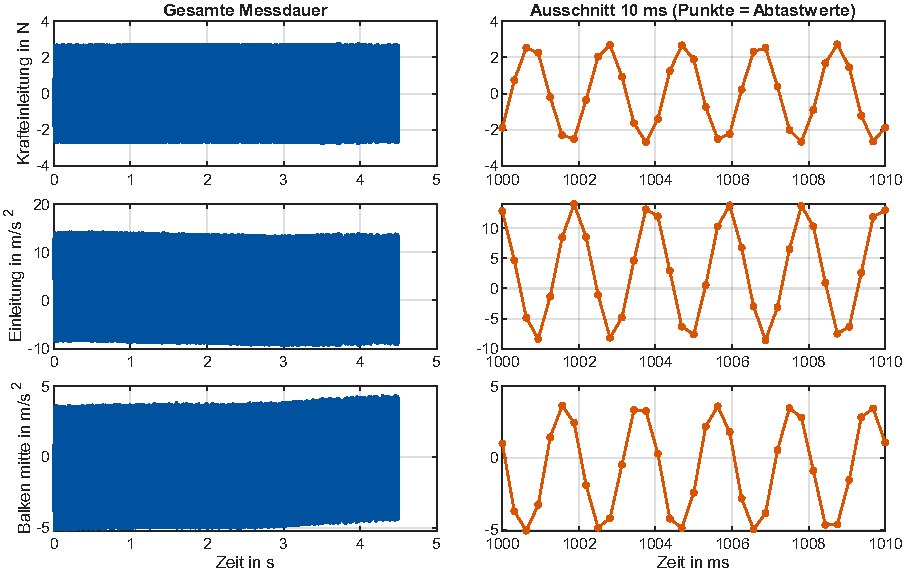
\includegraphics[width=\textwidth]{A0_zeit_500Hz}
  \caption{Zeitsignale bei Sinusanregung \SI{500}{\hertz} (Messung
  \texttt{T155748}). Links gesamte Messdauer, rechts Ausschnitt von
  \SI{10}{\milli\second} mit den einzelnen Abtastwerten.}
  \label{fig:zeit500}
\end{figure}

\begin{figure}[!htb]
  \centering
  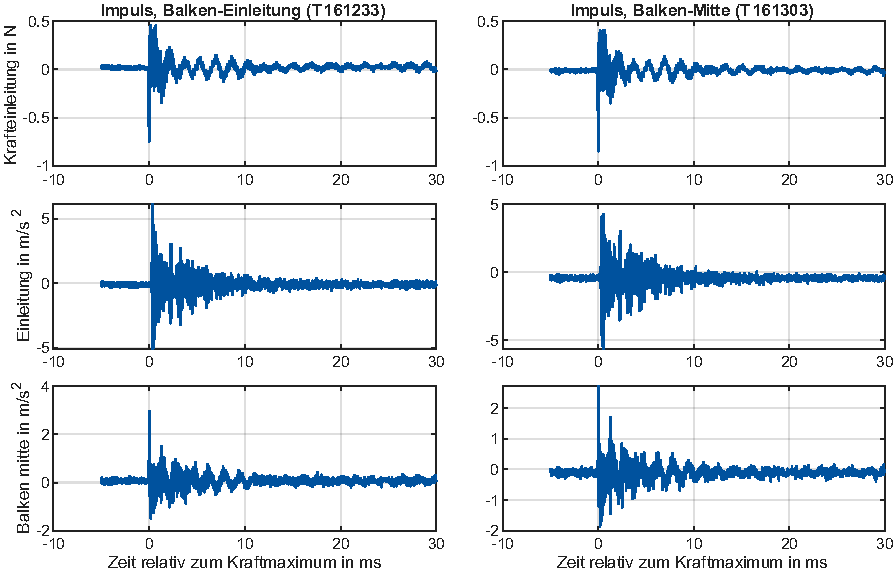
\includegraphics[width=\textwidth]{A0_zeit_impuls}
  \caption{Zeitsignale der beiden gültigen Impulsmessungen (Versuch~3) um den
  Zeitpunkt des Kraftmaximums.}
  \label{fig:zeitimpuls}
\end{figure}

\begin{figure}[!htb]
  \centering
  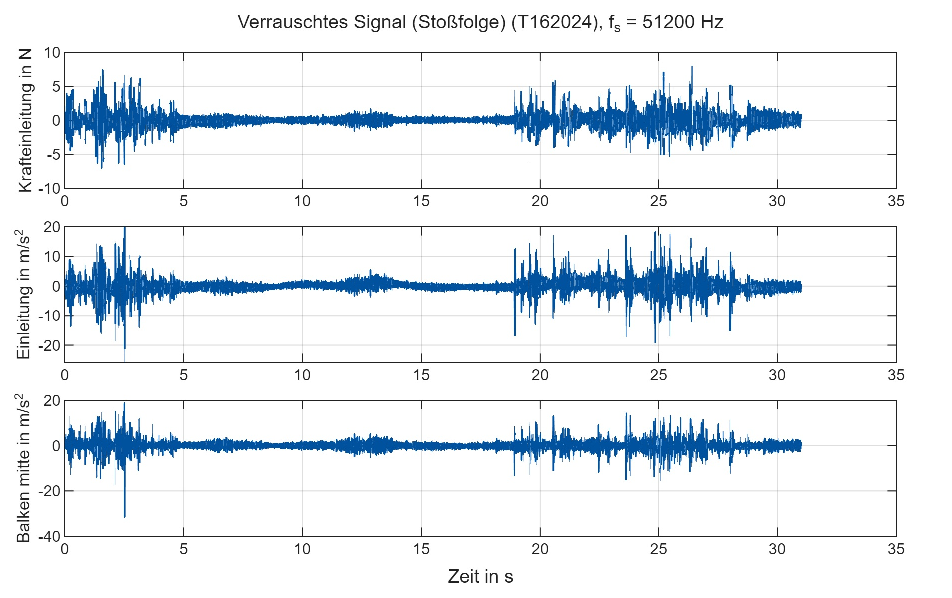
\includegraphics[width=\textwidth]{A0_zeit_rauschen}
  \caption{Zeitsignale des verrauschten Signals (Versuch~4).}
  \label{fig:zeitrauschen}
\end{figure}

\paragraph{Auswertung.} Die Auswertung erfolgt mit den MATLAB-Skripten im
Ordner \texttt{Auswertung\_MATLAB} (Anhang~\ref{sec:anhang}) und der Signal
Processing Toolbox. Die Spektren werden wie in der Versuchsunterlage
beschrieben mit einer Kurzzeit-FFT (\texttt{spectrogram}) berechnet:
$N=f_s/\Delta f$, Fensterfunktion (\texttt{rectwin}, \texttt{hann},
\texttt{flattopwin}), Überlappung $2/3$, $\Sx = 2|S|/(N F_M)$, $\Sxx = \Sx^2$,
$\Gxx$ als einseitige Leistungsdichte, lineare Mittelung über alle Blöcke.
Übertragungsfunktionen und Kohärenz werden mit \texttt{tfestimate} und
\texttt{mscohere} bestimmt. Alle Gleichanteile werden vor der Analyse entfernt.

% ==================================================================
\section{Ergebnisse und Diskussion}
% ==================================================================

% ------------------------------------------------------------------
\subsection{Einfluss der Abtastrate}
% ------------------------------------------------------------------

\paragraph{Messung mit drei Abtastraten.} \abb{fig:spektrenfs} zeigt die
Betragsspektren der Sinusanregung (Grundfrequenz \GrundFrequenz\,Hz) aus
Versuch~2. Mit \SI{12.8}{\kilo\hertz} und \SI{51.2}{\kilo\hertz} werden
Harmonische bis über \SI{5.5}{\kilo\hertz} sichtbar; der Erreger erzeugt also
keinen reinen Sinus. Bei $f_s=\SI{3200}{\hertz}$ ist der Frequenzbereich auf
$f_N=\SI{1600}{\hertz}$ begrenzt und nur die ersten drei Harmonischen sind
erfassbar. Die Amplituden aller erfassten Linien stimmen zwischen den drei
Messungen auf wenige Prozent überein (\tab{tab:harmonische}).

\begin{figure}[!htb]
  \centering
  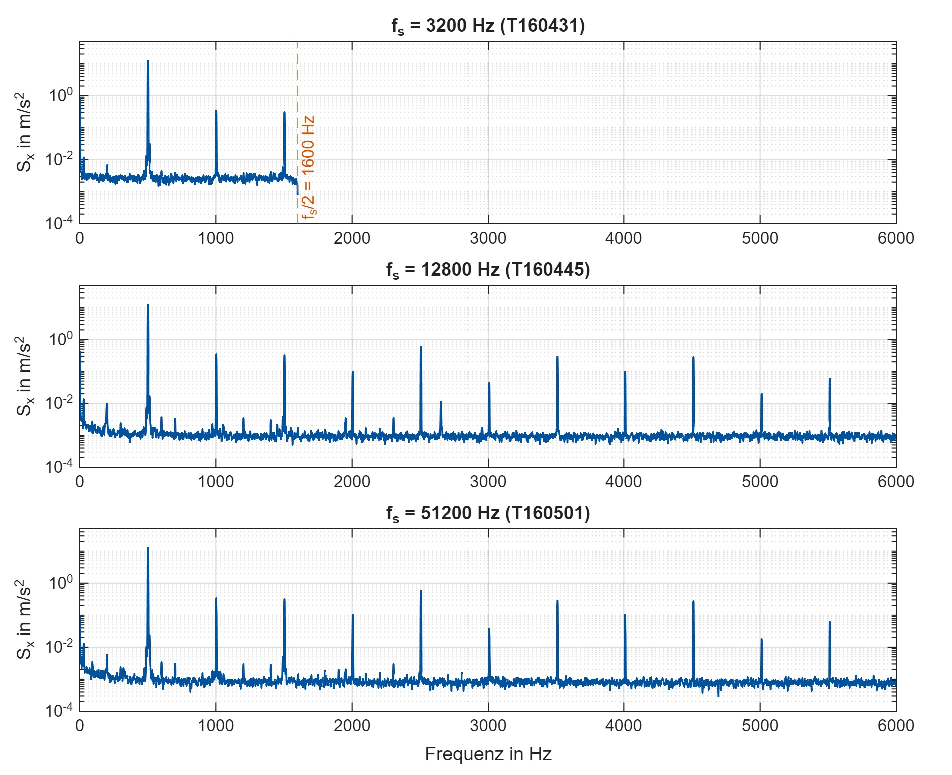
\includegraphics[width=\textwidth]{A1_spektren_fs}
  \caption{Betragsspektren (Einleitung, Flattop, $\Delta f=\SI{1}{\hertz}$)
  der Sinusanregung bei den drei gemessenen Abtastraten.}
  \label{fig:spektrenfs}
\end{figure}

\begin{table}[H]
  \centering
  \caption{Amplituden $\Sx$ der Harmonischen in \si{\metre\per\second\squared}
  (Einleitung, Flattop). --: oberhalb von $f_N$.}
  \label{tab:harmonische}
  \begin{tabular}{rrrrr}
    \toprule
    $k$ & $f_k$ in Hz & $f_s=\SI{3200}{\hertz}$ & $f_s=\SI{12800}{\hertz}$ & $f_s=\SI{51200}{\hertz}$ \\
    \midrule
    \tabinput{tab_harmonische}
    \bottomrule
  \end{tabular}
\end{table}

\paragraph{Aliasing.} Obwohl das Signal Harmonische oberhalb von
\SI{1600}{\hertz} enthält, zeigt die mit \SI{3200}{\hertz} gemessene Datei an
den nach Gl.~\eqref{eq:alias} zu erwartenden Alias-Frequenzen keine Linien
(\abb{fig:aliasing} unten, \tab{tab:aliasing} letzte Spalte). Das
Messsystem besitzt also ein wirksames Anti-Aliasing-Filter; bei
Delta-Sigma-Wandlern, wie sie in CompactDAQ-Modulen eingesetzt werden, ist
dieses als digitales Filter integriert und wird mit der Abtastrate
mitgeführt.

Um Aliasing trotzdem sichtbar zu machen, wird die \SI{51.2}{\kilo\hertz}-Messung
nachträglich auf \SI{3200}{\hertz} reduziert -- einmal durch bloßes Weglassen
von Werten (\texttt{downsample}, kein Filter), einmal mit vorgeschaltetem
Tiefpass (\texttt{resample}). Ohne Filter erscheinen alle Harmonischen
oberhalb von $f_N$ mit unveränderter Amplitude an ihren Alias-Frequenzen,
z.\,B.\ die 5.~Harmonische (\SI{2506}{\hertz}) mit
\SI{0.59}{\metre\per\second\squared} bei \SI{694}{\hertz}. Diese Linien sind
von echten Signalanteilen nicht zu unterscheiden und würden fälschlich als
Schwingungen bei 193, 309, 694, 810\,\ldots\,Hz interpretiert. Mit
AA-Filter sind sie um ein bis knapp drei Dekaden gedämpft und liegen im
Rauschen, ebenso wie in der direkt mit \SI{3200}{\hertz} gemessenen Datei.

\begin{figure}[!htb]
  \centering
  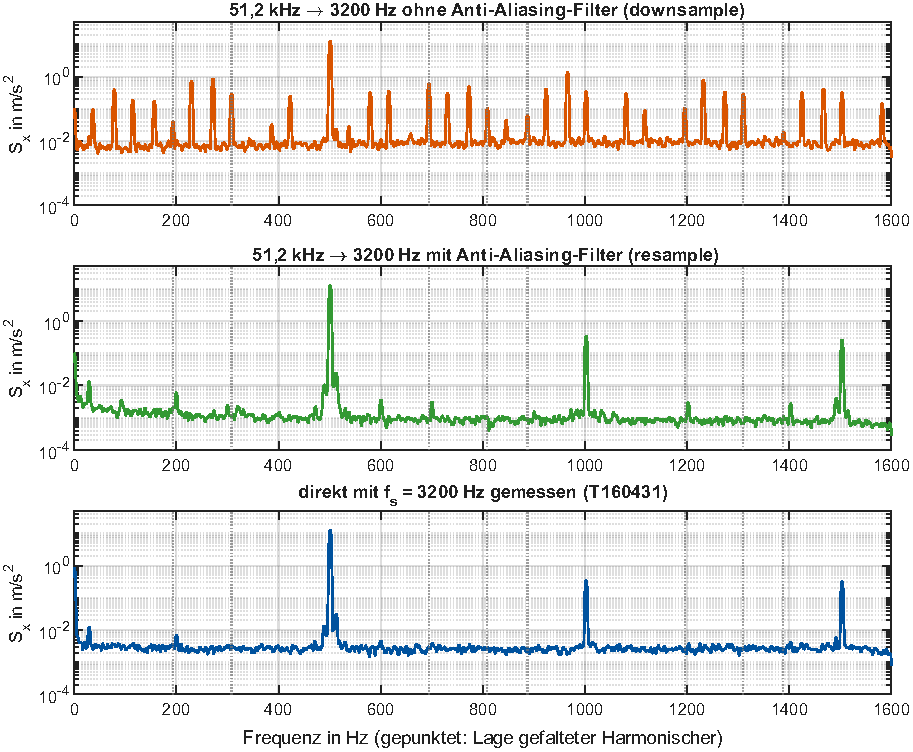
\includegraphics[width=\textwidth]{A1_aliasing}
  \caption{Betragsspektren bei $f_s=\SI{3200}{\hertz}$: nachträglich
  reduziert ohne (oben) bzw.\ mit Anti-Aliasing-Filter (Mitte) und direkt
  gemessen (unten). Gepunktet: Alias-Frequenzen der Harmonischen oberhalb von
  $f_N$.}
  \label{fig:aliasing}
\end{figure}

\begin{table}[H]
  \centering
  \caption{Harmonische oberhalb von $f_N=\SI{1600}{\hertz}$ und deren
  Amplitude $\Sx$ in \si{\metre\per\second\squared} an der Alias-Frequenz bei
  $f_s=\SI{3200}{\hertz}$.}
  \label{tab:aliasing}
  \small
  \begin{tabular}{rrrrrrr}
    \toprule
    $k$ & $f_k$ in Hz & $f_\text{alias}$ in Hz & $\Sx(f_k)$, \SI{51.2}{\kilo\hertz} & ohne Filter & mit Filter & gemessen \\
    \midrule
    \tabinput{tab_aliasing}
    \bottomrule
  \end{tabular}
\end{table}

\paragraph{Zeitbereich.} \abb{fig:aliasingzeit} zeigt dasselbe im Zeitbereich.
Bei \SI{51.2}{\kilo\hertz} liegen rund 100 Werte je Periode vor, bei
\SI{3200}{\hertz} nur 6,4: Die Frequenz ist noch korrekt erfasst, der
Spitzenwert wird aber nicht zuverlässig getroffen und der Verlauf wirkt
ungleichmäßig. Bei \SI{800}{\hertz} (jeder 64.~Wert) beschreiben die
Abtastwerte scheinbar eine Schwingung mit \SI{299}{\hertz} -- ohne Kenntnis
des Originalsignals wäre dies nicht als Fehler erkennbar.

\begin{figure}[!htb]
  \centering
  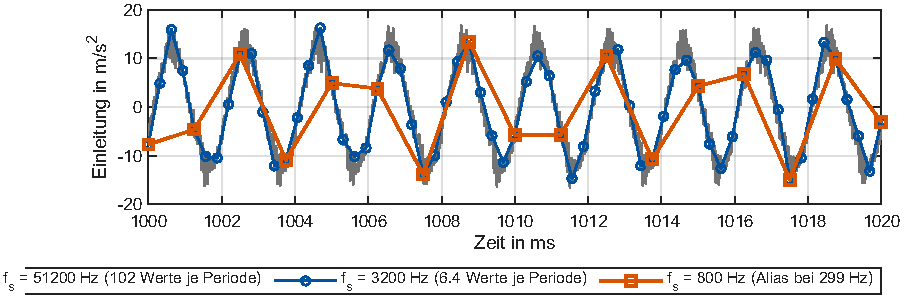
\includegraphics[width=\textwidth]{A1_aliasing_zeit}
  \caption{Zeitsignal der \SI{51.2}{\kilo\hertz}-Messung und daraus
  entnommene Abtastwerte für \SI{3200}{\hertz} und \SI{800}{\hertz}.}
  \label{fig:aliasingzeit}
\end{figure}

\paragraph{Impulse.} Der Kraftimpuls aus Versuch~3 ist bei
\SI{51.2}{\kilo\hertz} nur zwei Abtastwerte (ca.\ \SI{0.04}{\milli\second})
breit (\abb{fig:impuls}, \tab{tab:impuls}). Wird nur jeder 2., 4., 8.\ bzw.\
16.\ Wert verwendet, verfehlt das Raster das Maximum: Der Spitzenwert sinkt
von \SI{0.75}{\newton} auf \SI{0.43}{\newton}, und die ermittelte Impulsbreite
ist nur noch durch das Abtastintervall bestimmt. Wie stark der Spitzenwert
unterschätzt wird, hängt zufällig von der Lage des Abtastrasters ab.
\tab{tab:impulsstreuung} wertet alle möglichen Rasterlagen beider
Impulsmessungen und aller drei Kanäle aus: Bei \SI{3200}{\hertz} wird der
Spitzenwert im Mittel um \SI{47}{\percent} und im ungünstigsten Fall um
\SI{77}{\percent} zu niedrig erfasst. Impulsbehaftete Signale erfordern
daher hohe Abtastraten.

\begin{figure}[!htb]
  \centering
  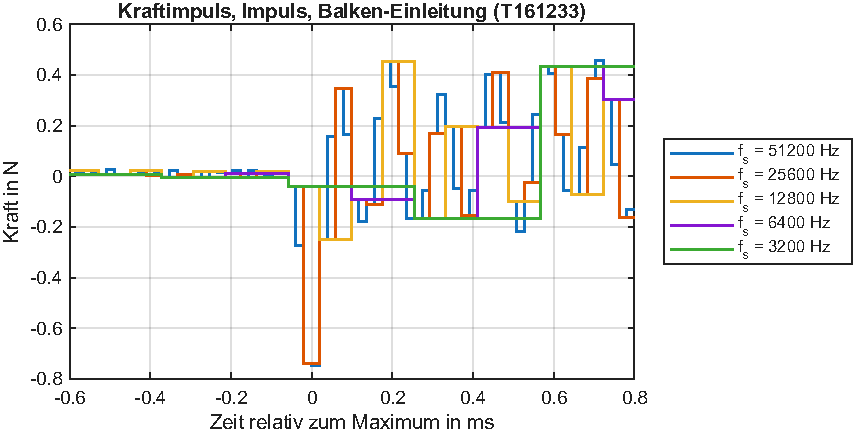
\includegraphics[width=\textwidth]{A1_impuls}
  \caption{Kraftimpuls bei unterschiedlichen Abtastraten, dargestellt als
  Treppenfunktion (Halteglied).}
  \label{fig:impuls}
\end{figure}

\begin{table}[H]
  \centering
  \begin{minipage}[t]{0.55\textwidth}
    \centering
    \captionof{table}{Spitzenwert und Impulsbreite (Werte $\ge\SI{50}{\percent}$
    des Spitzenwerts) des Kraftimpulses bei festem Abtastraster.}
    \label{tab:impuls}
    \small
    \begin{tabular}{rrrrr}
      \toprule
      $f_s$ & $\Delta t$ & $\hat F$ & Werte & Breite \\
      in Hz & in \si{\micro\second} & in N & & in ms \\
      \midrule
      \tabinput{tab_impuls}
      \bottomrule
    \end{tabular}
  \end{minipage}\hfill
  \begin{minipage}[t]{0.42\textwidth}
    \centering
    \captionof{table}{Unterschätzung des Spitzenwerts über alle Rasterlagen
    (2 Messungen, 3 Kanäle).}
    \label{tab:impulsstreuung}
    \small
    \begin{tabular}{rrr}
      \toprule
      $f_s$ & Mittel & Maximum \\
      in Hz & in \% & in \% \\
      \midrule
      \tabinput{tab_impuls_streuung}
      \bottomrule
    \end{tabular}
  \end{minipage}
\end{table}

\paragraph{Frequenzinhalt eines Impulses.} Ein so kurzer Impuls regt einen
sehr breiten Frequenzbereich an: Die Leistungsdichte der Kraft ist bis über
\SI{10}{\kilo\hertz} nahezu konstant (\abb{fig:spek51k}, oben), rund
\AnteilUeber\,\% der Leistung liegen oberhalb von \SI{1600}{\hertz}. Ohne
AA-Filter würden diese Anteile bei \SI{3200}{\hertz} in den Messbereich
gespiegelt und die Leistung im Band bis \SI{1280}{\hertz} um den Faktor
\AliasFaktor{} erhöhen (\abb{fig:spek51k}, unten). Da das gespiegelte
Spektrum hier ebenfalls flach ist, ist der Fehler -- anders als bei den
diskreten Linien oben -- nicht an der Form, sondern nur am Pegel erkennbar.

\begin{figure}[!htb]
  \centering
  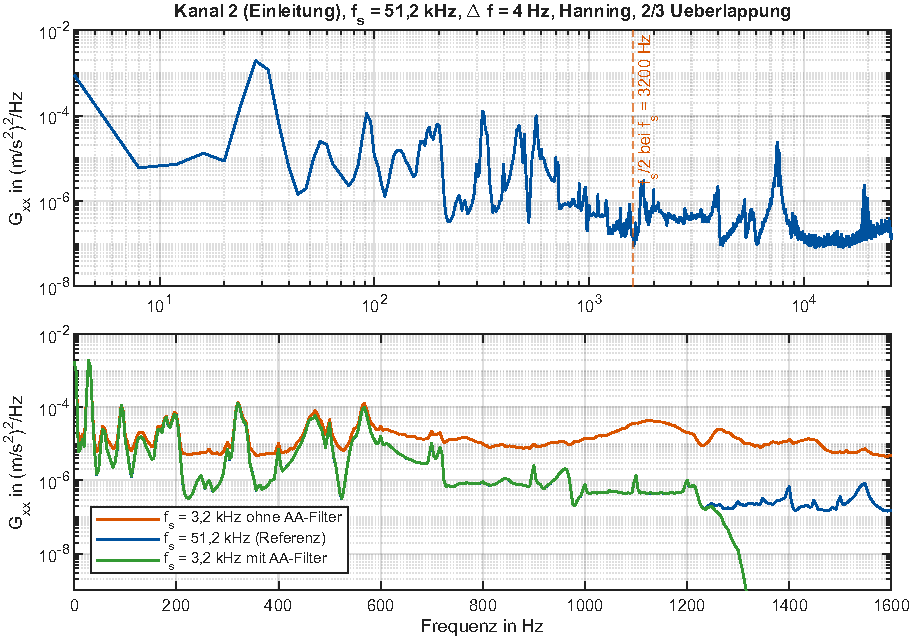
\includegraphics[width=\textwidth]{A1_spektrum_51k}
  \caption{Oben: Leistungsdichte des Kraftimpulses bei
  \SI{51.2}{\kilo\hertz} (\SI{0.5}{\second} ab dem Impuls). Unten: Vergleich
  mit Abtastung bei \SI{3.2}{\kilo\hertz} ohne bzw.\ mit Anti-Aliasing-Filter.}
  \label{fig:spek51k}
\end{figure}

\paragraph{Fazit Abtastrate.} Die Abtastrate legt den analysierbaren
Frequenzbereich fest ($f_s/2$, praktisch $f_s/2{,}56$). Zu niedrige
Abtastraten führen ohne AA-Filter zu Aliasing, das nachträglich nicht
erkennbar und nicht korrigierbar ist, und bei Impulsen zu falschen
Spitzenwerten und Impulsdauern. Das verwendete Messsystem filtert
vorbildlich; wird die Abtastrate jedoch nachträglich in Software reduziert,
muss selbst gefiltert werden. Hohe Abtastraten erzeugen große Datenmengen
(Versuch~4: 1,59~Mio.\ Werte je Kanal in \SI{31}{\second}). Sinnvoll ist
eine Orientierungsmessung mit hoher Abtastrate und die anschließende
Anpassung an den Bedarf.

% ------------------------------------------------------------------
\subsection{Einfluss der Fensterfunktion}
% ------------------------------------------------------------------

\paragraph{Eigenschaften der Fenster.} \abb{fig:fenstereig} zeigt die drei
untersuchten Fensterfunktionen und ihre Spektren, \tab{tab:fenster} die
Kennwerte. Das Rechteckfenster hat die schmalste Hauptkeule, aber hohe
Nebenkeulen (\SI{-13}{\decibel}). Das Hanning-Fenster dämpft die Nebenkeulen
stark (\SI{-31.5}{\decibel}, danach schneller Abfall), verbreitert die
Hauptkeule aber auf $B_\text{eff} = 1{,}5\,\Delta f$. Das Flattop-Fenster hat
eine sehr breite, oben flache Hauptkeule ($B_\text{eff} = 3{,}77\,\Delta f$)
und praktisch keinen Amplitudenfehler.

\begin{figure}[!htb]
  \centering
  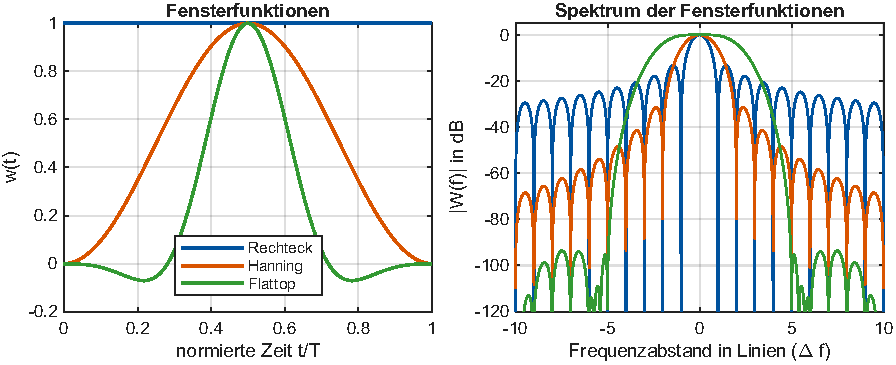
\includegraphics[width=\textwidth]{A2_fenster_eigenschaften}
  \caption{Fensterfunktionen (links) und deren Betragsspektren in dB über dem
  Frequenzabstand in Linien (rechts).}
  \label{fig:fenstereig}
\end{figure}

\begin{table}[H]
  \centering
  \caption{Kennwerte der Fensterfunktionen (berechnet für $N=3200$). Der
  maximale Amplitudenfehler gilt für ein Signal genau zwischen zwei Linien.}
  \label{tab:fenster}
  \begin{tabular}{lrrrrr}
    \toprule
    Fenster & $F_M$ & $P_M$ & $B_\text{eff}\cdot T$ & max.\ Amplitudenfehler & höchste Nebenkeule \\
            &       &       &                       & in dB                   & in dB \\
    \midrule
    \tabinput{tab_fenster}
    \bottomrule
  \end{tabular}
\end{table}

Die berechneten Werte entsprechen der Theorie: Hanning hat bis
\SI{1.42}{\decibel} Amplitudenfehler (vgl.\ \cite{esefeld}); das
MATLAB-Flattop-Fenster liegt mit \SI{0.01}{\decibel} sogar noch unter dem in
der Unterlage genannten Wert von \SI{0.19}{\decibel}.

\paragraph{Anwendung auf die Messung.} Die \SI{500}{\hertz}-Messung aus
Versuch~1 (\texttt{T155748}, \SI{4.5}{\second}) wird mit allen drei Fenstern
in zwei Fällen ausgewertet (\abb{fig:fenstermess}, \tab{tab:fenstermess}):
\begin{itemize}
  \item \textbf{Fall A} ($N=3200$, $\Delta f=\SI{1}{\hertz}$): Jeder Block
        enthält genau 500 Perioden, \SI{500}{\hertz} liegt exakt auf einer
        Linie. Alle Fenster liefern dieselbe Amplitude
        (\SI{11.0}{\metre\per\second\squared}). Das Rechteckfenster ist hier
        sogar optimal, da kein Leckeffekt auftritt und die Linie am
        schmalsten ist.
  \item \textbf{Fall B} ($N=1072$, $\Delta f=\SI{2.985}{\hertz}$): Jeder Block
        enthält 167,5 Perioden, \SI{500}{\hertz} liegt genau zwischen zwei
        Linien (ungünstigster Fall). Das Rechteckfenster unterschätzt die
        Amplitude um \SI{36}{\percent}, Hanning um \SI{15}{\percent}, Flattop
        nur um \SI{0.2}{\percent}; für die 3.~Harmonische ergibt sich
        dasselbe Bild. Zusätzlich hebt der Leckeffekt beim Rechteckfenster
        den Rauschboden in der Umgebung der Linie um rund zwei Dekaden an;
        schwache Anteile gehen im Leck der starken Linie unter. Mit Hanning
        und Flattop bleibt die Dynamik erhalten.
\end{itemize}
Die Messung bestätigt damit die theoretischen Werte aus \tab{tab:fenster}.
\abb{fig:fensterzeit} zeigt die Ursache: Beim Rechteckfenster entstehen an
den Blockgrenzen Sprünge im periodisch fortgesetzten Signal, Hanning und
Flattop führen das Signal stetig gegen null.

\begin{figure}[!htb]
  \centering
  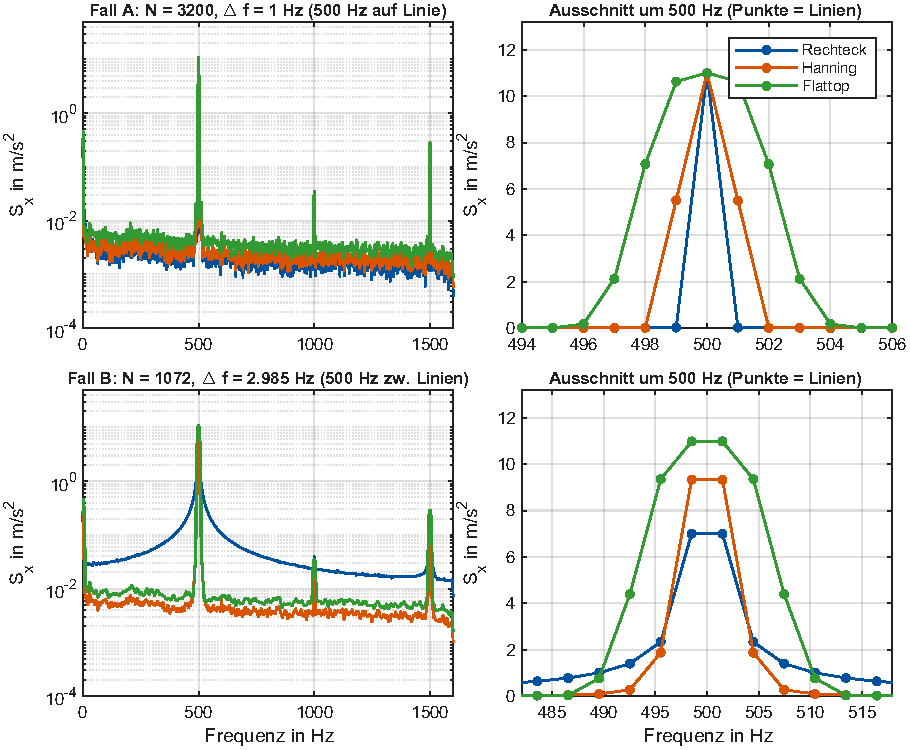
\includegraphics[width=\textwidth]{A2_fenster_messung}
  \caption{Betragsspektren der \SI{500}{\hertz}-Messung (Einleitung) mit
  verschiedenen Fenstern. Oben: Signalfrequenz auf einer Linie, unten:
  Signalfrequenz zwischen zwei Linien. Rechts Ausschnitt um \SI{500}{\hertz}
  (Punkte = Spektrallinien).}
  \label{fig:fenstermess}
\end{figure}

\begin{table}[H]
  \centering
  \caption{Gemessene Amplituden $\Sx$ in \si{\metre\per\second\squared} bei
  \SI{500}{\hertz} und \SI{1500}{\hertz}. Abweichung von Fall B bezogen auf
  Flattop, Fall A.}
  \label{tab:fenstermess}
  \begin{tabular}{lrrrrrr}
    \toprule
     & \multicolumn{3}{c}{\SI{500}{\hertz}} & \multicolumn{3}{c}{\SI{1500}{\hertz}} \\
    \cmidrule(lr){2-4}\cmidrule(lr){5-7}
    Fenster & Fall A & Fall B & Abw.\ in \% & Fall A & Fall B & Abw.\ in \% \\
    \midrule
    \tabinput{tab_fenster_messung}
    \bottomrule
  \end{tabular}
\end{table}

\begin{figure}[!htb]
  \centering
  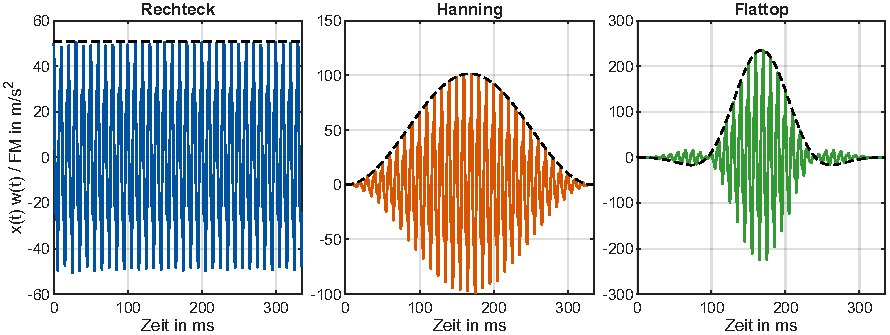
\includegraphics[width=\textwidth]{A2_fenster_zeit}
  \caption{Ein Block (Fall B) nach Multiplikation mit der Fensterfunktion und
  Amplitudenkorrektur $1/F_M$; gestrichelt die skalierte Fensterfunktion.}
  \label{fig:fensterzeit}
\end{figure}

\paragraph{Fazit Fensterfunktion.} Die Fensterfunktion bestimmt den
Kompromiss zwischen Amplitudengenauigkeit, Frequenzselektivität und Dynamik.
Rechteck nur bei Signalen, die exakt periodisch im Block sind, oder bei
Impulsen, die vollständig im Block abklingen (Versuch~3). Hanning als
Standard für unbekannte bzw.\ breitbandige Signale. Flattop für die genaue
Amplitudenbestimmung sinusförmiger Signale. Ergebnisse sind nur bei gleicher
Fensterung vergleichbar.

% ------------------------------------------------------------------
\subsection{Einfluss der Frequenzauflösung}
% ------------------------------------------------------------------

\paragraph{Periodisches Signal.} \abb{fig:aufloesungsinus} und
\tab{tab:aufloesung} zeigen die \SI{500}{\hertz}-Messungen aus Versuch~1,
jeweils mit der bei der Messung eingestellten Auflösung $\Delta f = 0{,}25$,
1 und \SI{4}{\hertz} ausgewertet (Hanning). Die Amplitude der Linie ist
unabhängig von $\Delta f$ (\SI{11.4}{\metre\per\second\squared}), die
Linienbreite skaliert dagegen mit $\Delta f$. Gleichzeitig wächst die nötige
Blockdauer $T=1/\Delta f$: Bei $\Delta f=\SI{0.25}{\hertz}$ ist ein Block
\SI{4}{\second} lang, sodass die \SI{4.5}{\second} lange Messung nur
\emph{einen} Block ohne Mittelung liefert; bei \SI{4}{\hertz} sind es 52
Mittelungen. Genau an diesem Zusammenhang scheiterte die ausgeschiedene
Messung \texttt{T155705}: Mit \SI{3.5}{\second} ist sie kürzer als ein Block
und mit \SI{0.25}{\hertz} gar nicht auswertbar. Der Rauschboden von $\Sx$
steigt mit $\sqrt{\Delta f}$, da in eine breitere Linie mehr Rauschleistung
fällt.

\begin{figure}[!htb]
  \centering
  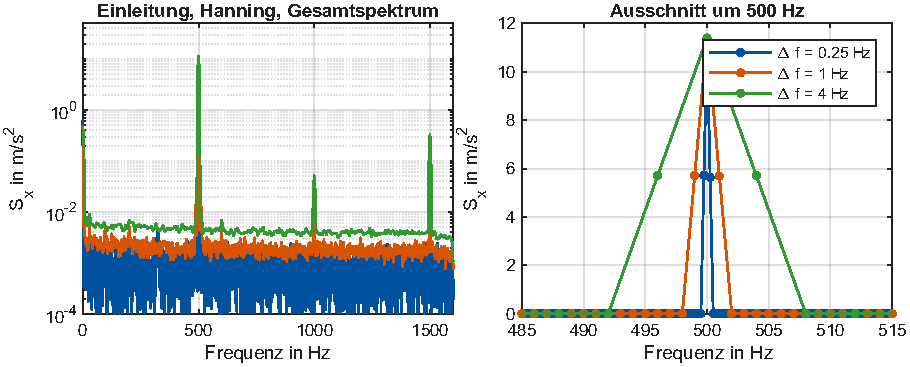
\includegraphics[width=\textwidth]{A3_aufloesung_sinus}
  \caption{Betragsspektrum der \SI{500}{\hertz}-Messungen (Einleitung,
  Hanning) bei verschiedenen Frequenzauflösungen.}
  \label{fig:aufloesungsinus}
\end{figure}

\begin{table}[H]
  \centering
  \caption{Parameter der Analyse (Hanning, \SI{66.7}{\percent} Überlappung).
  $T_\text{mess}$: Messdauer, $T$: Blockdauer.}
  \label{tab:aufloesung}
  \small
  \begin{tabular}{rlrrrrrr}
    \toprule
    $\Delta f$ in Hz & Messung & $T_\text{mess}$ in s & $N$ & $T$ in s & $n_d$ & $B_\text{eff}$ in Hz & $\Sx(\SI{500}{\hertz})$ in \si{\metre\per\second\squared} \\
    \midrule
    \tabinput{tab_aufloesung}
    \bottomrule
  \end{tabular}
\end{table}

\paragraph{Auflösung von Resonanzen.} \abb{fig:aufloesungres} zeigt den
Betrag der Übertragungsfunktion Balkenmitte/Kraft aus einer Impulsmessung,
berechnet aus einem einzigen Block ab dem Impuls mit Blockdauern zwischen
\SI{62.5}{\milli\second} und \SI{4}{\second}. Mit $\Delta f = \SI{16}{\hertz}$
ist die Kurve glatt, Resonanzspitzen werden aber verbreitert und abgeflacht;
eng benachbarte Spitzen (z.\,B.\ im Ausschnitt um \SI{530}{\hertz}) verschmelzen.
Feinere Auflösung bildet die Spitzen schärfer ab, die Kurven werden jedoch
zunehmend verrauscht: Die Antwort ist nach etwa \SI{50}{\milli\second}
abgeklungen, ein längerer Block fügt nur noch Messrauschen hinzu. Beim
Impulsversuch ist die im Protokoll eingestellte Auflösung von
\SI{0.25}{\hertz} daher ungünstig; die Blockdauer sollte an die Abklingzeit
angepasst werden.

\begin{figure}[!htb]
  \centering
  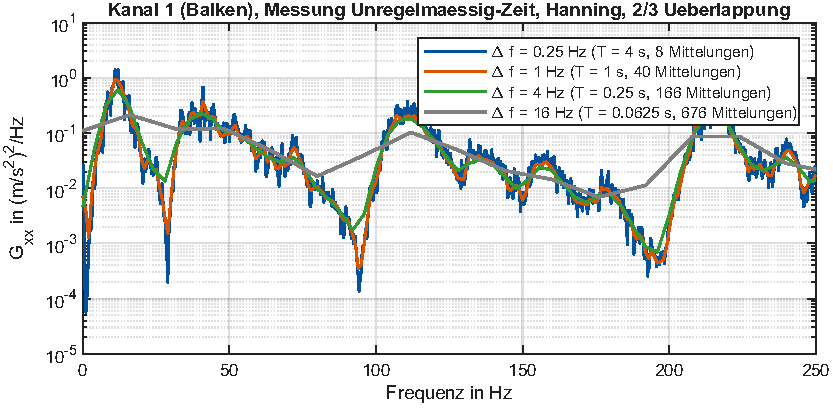
\includegraphics[width=\textwidth]{A3_aufloesung_resonanzen}
  \caption{Betrag der Übertragungsfunktion Balkenmitte/Kraft (Messung
  \texttt{T161303}) bei verschiedenen Frequenzauflösungen (ein Block,
  Rechteckfenster). Unten Ausschnitt 450\ldots\SI{650}{\hertz}.}
  \label{fig:aufloesungres}
\end{figure}

\paragraph{Zeit-Frequenz-Unschärfe.} Beim verrauschten Signal mit
wechselnder Stoßintensität wird der Zielkonflikt nach
Gl.~\eqref{eq:unschaerfe} sichtbar (\abb{fig:spektrogramm}). Mit
$\Delta f=\SI{0.5}{\hertz}$ ($T=\SI{2}{\second}$) sind die Frequenzen fein
aufgelöst, die zeitliche Struktur (Wechsel zwischen ruhigen und intensiven
Abschnitten) ist aber über rund \SI{2}{\second} verschmiert. Mit
$\Delta f=\SI{32}{\hertz}$ ($T=\SI{31.25}{\milli\second}$) sind sogar einzelne
Stöße als senkrechte Linien erkennbar, die Frequenzen verschwimmen jedoch zu
\SI{32}{\hertz} breiten Bändern. Beides gleichzeitig beliebig genau zu
bestimmen ist nicht möglich.

\begin{figure}[!htb]
  \centering
  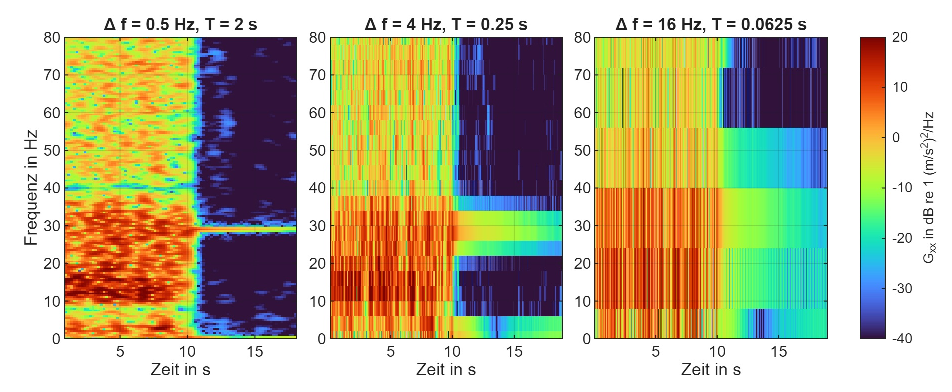
\includegraphics[width=\textwidth]{A3_spektrogramm}
  \caption{Spektrogramme (Leistungsdichte in dB, Einleitung, Hanning,
  \SI{90}{\percent} Überlappung) des verrauschten Signals bei verschiedenen
  Frequenzauflösungen.}
  \label{fig:spektrogramm}
\end{figure}

\paragraph{Fazit Frequenzauflösung.} Die Frequenzauflösung legt über
$T = 1/\Delta f$ die Blockdauer fest. Feine Auflösung trennt benachbarte
Frequenzen, benötigt aber lange stationäre Messungen und liefert bei gegebener
Messdauer wenige Mittelungen sowie eine schlechte Zeitauflösung. Bei
abklingenden Vorgängen erhöht ein zu langer Block nur das Rauschen. Grobe
Auflösung verschmiert Frequenzen, erlaubt aber viele Mittelungen und das
Verfolgen zeitlicher Änderungen. $\Delta f$ und Messdauer müssen gemeinsam an
Signal und Fragestellung angepasst werden.

% ------------------------------------------------------------------
\subsection{Einfluss der Spektraldarstellung}
% ------------------------------------------------------------------

\paragraph{Variation der Frequenzauflösung.} \abb{fig:sxsxxgxx} stellt
$\Sx$, $\Sxx$ und $\Gxx$ eines periodischen (links, Sinus \SI{500}{\hertz})
und eines breitbandigen Signals (rechts, verrauschtes Signal) für drei
Frequenzauflösungen gegenüber, \tab{tab:spektrendf} fasst die Kennwerte
zusammen:
\begin{itemize}
  \item \textbf{Betragsspektrum $\Sx$:} Die Amplitude der periodischen Linie
        ist unabhängig von $\Delta f$ (\SI{11.0}{\metre\per\second\squared})
        und entspricht direkt der Sinusamplitude. Der Rauschboden und das
        gesamte breitbandige Spektrum steigen dagegen mit $\sqrt{\Delta f}$
        (Faktor 2 je Vervierfachung).
  \item \textbf{Autoleistungsspektrum $\Sxx$:} Quadrat von $\Sx$; die
        Linienwerte sind konstant (Amplitude$^2$), der breitbandige Anteil
        steigt proportional zu $\Delta f$. Durch das Quadrieren treten
        energiereiche Bereiche stärker hervor.
  \item \textbf{Leistungsdichte $\Gxx$:} Der breitbandige Anteil und der
        Rauschboden sind unabhängig von $\Delta f$ (die drei Kurven rechts
        liegen übereinander). Die Höhe der periodischen Linie skaliert
        dagegen mit $1/B_\text{eff}$ (161, 40 und
        \SI{10}{(\metre\per\second\squared)^2\per\hertz}), da die gesamte
        Leistung des Sinus auf eine Linie der Breite $B_\text{eff}$ verteilt
        wird.
\end{itemize}

\begin{figure}[!htb]
  \centering
  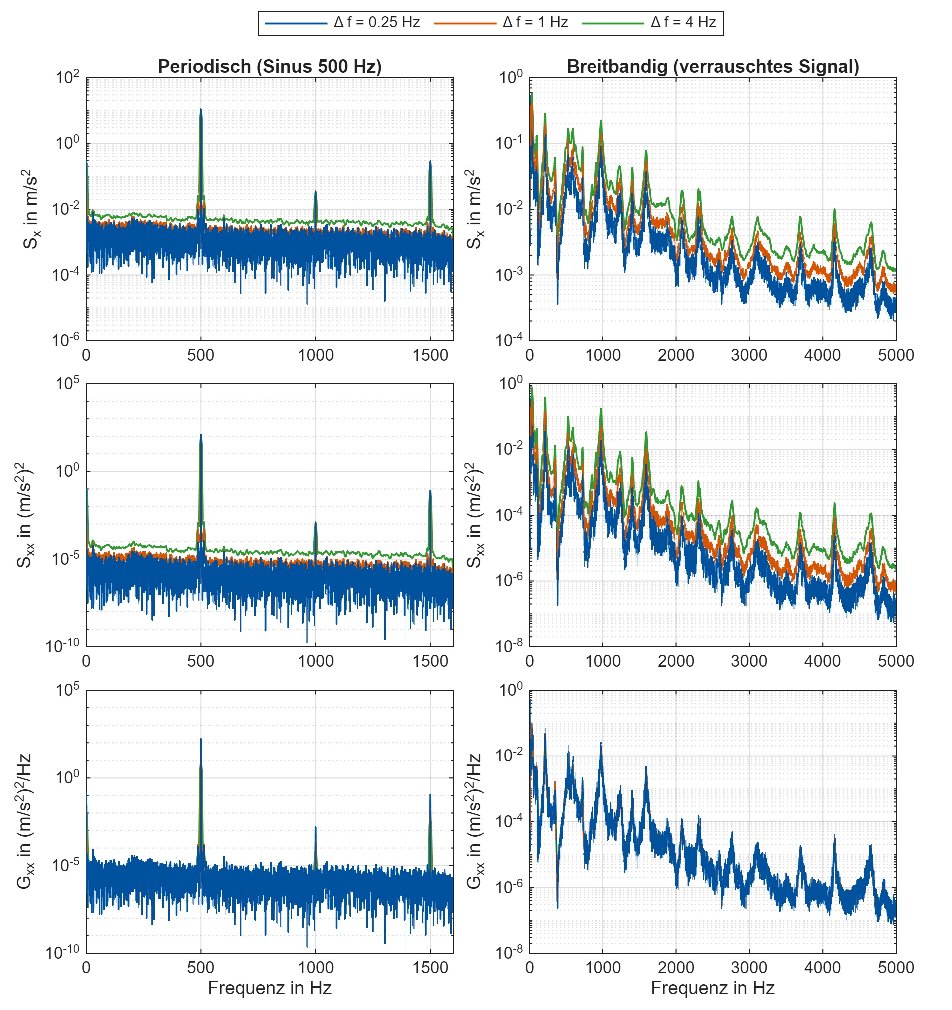
\includegraphics[width=\textwidth]{A4_sx_sxx_gxx}
  \caption{$\Sx$, $\Sxx$ und $\Gxx$ (Einleitung, Hanning) eines periodischen
  (links, \texttt{T155748}) und eines breitbandigen Signals (rechts,
  \texttt{T162024}) bei verschiedenen Frequenzauflösungen.}
  \label{fig:sxsxxgxx}
\end{figure}

\begin{table}[H]
  \centering
  \caption{Wert der \SI{500}{\hertz}-Linie und Median des Rauschbodens
  (1100\ldots\SI{1400}{\hertz}) für die drei Spektraldarstellungen (Hanning).}
  \label{tab:spektrendf}
  \small
  \begin{tabular}{rrrrrrr}
    \toprule
     & \multicolumn{3}{c}{Linie \SI{500}{\hertz}} & \multicolumn{3}{c}{Rauschboden} \\
    \cmidrule(lr){2-4}\cmidrule(lr){5-7}
    $\Delta f$ in Hz & $\Sx$ in \si{\metre\per\second\squared} & $\Sxx$ in \si{(\metre\per\second\squared)^2} & $\Gxx$ in \si{(\metre\per\second\squared)^2\per\hertz}
                     & $\Sx$ & $\Sxx$ & $\Gxx$ \\
    \midrule
    \tabinput{tab_spektren_df}
    \bottomrule
  \end{tabular}
\end{table}

Der etwas geringere Rauschboden von $\Gxx$ bei $\Delta f=\SI{0.25}{\hertz}$
ist eine Folge der fehlenden Mittelung (nur ein Block): Der Median eines
ungemittelten Rauschspektrums liegt systematisch unter dessen Mittelwert.

\paragraph{Variation der Fensterfunktion.} Dasselbe Verhalten zeigt sich bei
Variation des Fensters (\abb{fig:fenstersxgxx}, \tab{tab:spektrenfenster}):
$\Sx$ liefert für die periodische Linie mit allen Fenstern dieselbe Amplitude,
$\Gxx$ dagegen fällt mit wachsendem $B_\text{eff}$. Beim breitbandigen Signal
ist es umgekehrt: $\Gxx$ ist nahezu fensterunabhängig, $\Sx$ steigt mit
$\sqrt{B_\text{eff}/\Delta f}$ (Hanning $\times 1{,}18$, Flattop
$\times 1{,}85$ gegenüber Rechteck).

\begin{figure}[!htb]
  \centering
  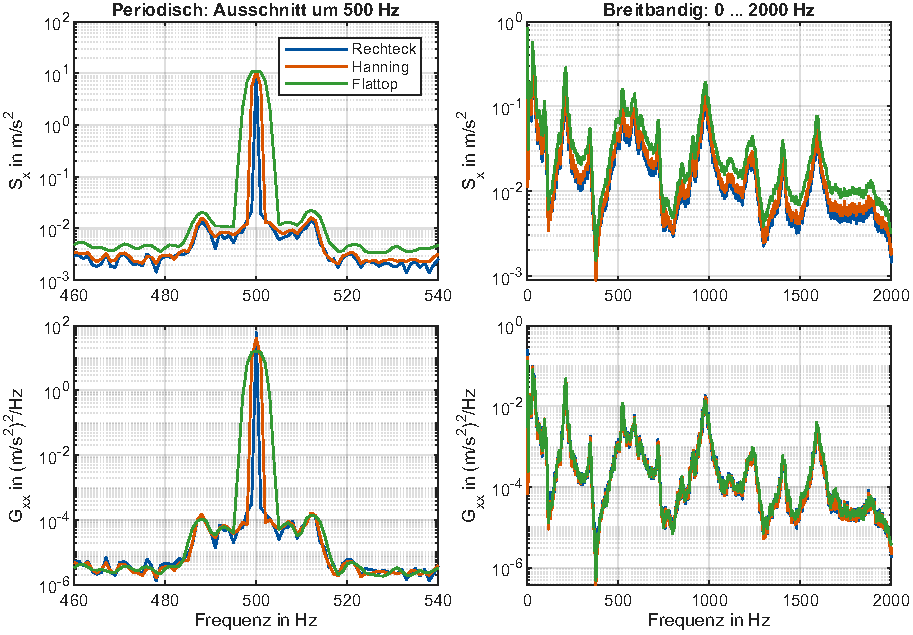
\includegraphics[width=\textwidth]{A4_fenster_sx_gxx}
  \caption{$\Sx$ (oben) und $\Gxx$ (unten) mit verschiedenen Fenstern bei
  $\Delta f=\SI{1}{\hertz}$; links periodisches, rechts breitbandiges Signal.}
  \label{fig:fenstersxgxx}
\end{figure}

\begin{table}[H]
  \centering
  \caption{Einfluss des Fensters ($\Delta f=\SI{1}{\hertz}$): periodische Linie
  bei \SI{500}{\hertz} und Mittelwert des breitbandigen Signals im Bereich
  200\ldots\SI{1000}{\hertz}.}
  \label{tab:spektrenfenster}
  \begin{tabular}{lrrrrr}
    \toprule
     & & \multicolumn{2}{c}{periodisch, \SI{500}{\hertz}} & \multicolumn{2}{c}{breitbandig, 200\ldots\SI{1000}{\hertz}} \\
    \cmidrule(lr){3-4}\cmidrule(lr){5-6}
    Fenster & $B_\text{eff}$ in Hz & $\Sx$ & $\Gxx$ & $\Sx$ & $\Gxx$ \\
    \midrule
    \tabinput{tab_spektren_fenster}
    \bottomrule
  \end{tabular}
\end{table}

\paragraph{Energiebilanz.} Nach Parseval muss die Fläche unter $\Gxx$ dem
Quadrat des Effektivwerts entsprechen. \tab{tab:parseval} bestätigt dies für
das periodische Signal mit allen Fenstern auf \SI{0.1}{\percent}. Beim
verrauschten Signal liegen die Abweichungen bei bis zu \SI{5}{\percent}:
Durch die Überlappung werden die Werte am Anfang und Ende der Messung
geringer gewichtet, und gerade dort treten kräftige Stöße auf; das Signal ist
nicht stationär. Wird der Effektivwert dagegen aus $\Sxx$ berechnet, ist er
nur beim Rechteckfenster korrekt und wird sonst um den Faktor
$\sqrt{B_\text{eff}/\Delta f}$ überschätzt (Hanning $\sqrt{1{,}5}$, Flattop
$\sqrt{3{,}77}$). Die Amplitudenkorrektur mit $F_M$ verfälscht also die
Signalenergie -- wie in der Versuchsunterlage angegeben.

\begin{table}[H]
  \centering
  \caption{Effektivwert der Beschleunigung an der Einleitung in
  \si{\metre\per\second\squared} aus dem Zeitsignal und aus den Spektren
  ($\Delta f=\SI{1}{\hertz}$).}
  \label{tab:parseval}
  \begin{tabular}{llrrr}
    \toprule
    Signal & Fenster & $\tilde x$ (Zeit) & $\sqrt{\sum \Gxx\,\Delta f}$ & $\sqrt{\sum \Sxx/2}$ \\
    \midrule
    \tabinput{tab_parseval}
    \bottomrule
  \end{tabular}
\end{table}

\paragraph{Fazit Spektraldarstellung.} $\Sx$ eignet sich für periodische
(diskrete) Signale, da Amplituden direkt ablesbar sind; die Werte
breitbandiger Anteile hängen jedoch von $\Delta f$ und Fenster ab. $\Sxx$
betont energiereiche Frequenzbereiche, ist aber ebenso parameterabhängig.
$\Gxx$ ist für breitbandige und stochastische Signale die geeignete
Darstellung, da sie unabhängig von den FT-Parametern ist und Vergleiche
zwischen verschiedenen Einstellungen und Analysatoren erlaubt; für Sinus-Linien
ist der Zahlenwert dagegen parameterabhängig. Die Wahl der Darstellung muss
daher stets mit angegeben werden.

% ------------------------------------------------------------------
\subsection{Einfluss der Sensorposition}\label{sec:position}
% ------------------------------------------------------------------

\paragraph{Erwartung.} Beim Kragbalken liegt das freie Ende für alle
Biegeeigenformen in einem Schwingungsbauch. Der Sensor nahe dem
Krafteinleitungspunkt misst daher annähernd die Antwort im Anregungspunkt
selbst (Punktübertragungsfunktion): Resonanzen und Antiresonanzen wechseln
sich hier ab, und in einer Antiresonanz bewegt sich der Anregungspunkt kaum,
obwohl der übrige Balken schwingt. Die Balkenmitte liegt dagegen je nach
Eigenform im Bauch oder in der Nähe eines Knotens. Für den idealen Kragbalken
(ohne Zusatzmasse von Erreger und Kraftsensor) liegen die Knoten, gemessen von
der Einspannung, bei $x/L \approx 0{,}78$ (2.~Eigenform), $0{,}50$ und $0{,}87$
(3.~Eigenform) sowie $0{,}36$, $0{,}64$ und $0{,}91$ (4.~Eigenform)
(Lösung der Euler-Bernoulli-Balkengleichung). Der Sensor in der Balkenmitte sitzt also praktisch im Knoten
der 3.~Eigenform und kann diese kaum erfassen.

\paragraph{Sinusanregung.} \abb{fig:positionen} vergleicht die
Betragsspektren an der Einleitung und in der Balkenmitte bei Sinusanregung
mit \SI{51.2}{\kilo\hertz} (Flattop, um Amplitudenfehler auszuschließen).
Beide Sensoren erfassen dieselben Frequenzen, aber mit deutlich
unterschiedlichen Amplituden, und das Verhältnis hängt stark von der Frequenz
ab (\tab{tab:positionen}): Die Grundschwingung erreicht die Balkenmitte nur
mit \SI{39}{\percent} (\SI{-8}{\decibel}) der Amplitude an der Einleitung,
die 3.~Harmonische bei \SI{1503}{\hertz} dagegen mit dem Sechsfachen
(\SI{+16}{\decibel}). An der Einleitung ist die 3.~Harmonische mit
\SI{0.32}{\metre\per\second\squared} unbedeutend, in der Balkenmitte ist sie
mit \SI{1.9}{\metre\per\second\squared} nach der Grundschwingung die
zweitstärkste Linie. Das Spektrum in der Balkenmitte ist damit keine
skalierte Kopie des Anregungsspektrums; die Rangfolge der Harmonischen
ändert sich.

\begin{figure}[!htb]
  \centering
  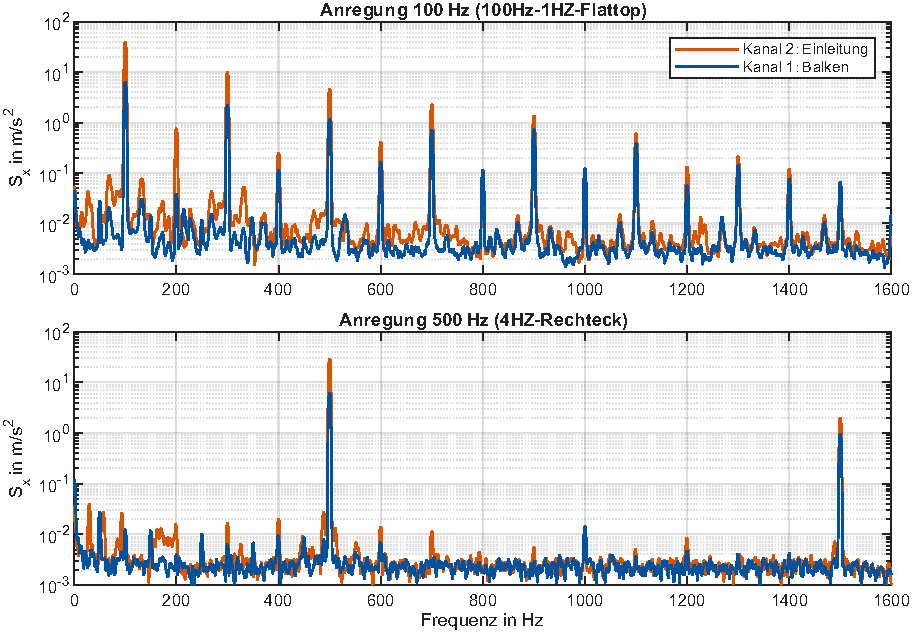
\includegraphics[width=\textwidth]{A5_spektren_positionen}
  \caption{Betragsspektren (Flattop, $\Delta f=\SI{1}{\hertz}$) an der
  Einleitung und in der Balkenmitte bei Sinusanregung (\texttt{T160501}).}
  \label{fig:positionen}
\end{figure}

\begin{table}[H]
  \centering
  \caption{Amplituden $\Sx$ in \si{\metre\per\second\squared} der
  Harmonischen an beiden Sensorpositionen und deren Verhältnis
  $|T| = S_{x,\text{Mitte}}/S_{x,\text{Einl.}}$ (nur deutliche Linien).}
  \label{tab:positionen}
  \begin{tabular}{rrrrrr}
    \toprule
    $k$ & $f$ in Hz & Einleitung & Mitte & $|T|$ & $|T|$ in dB \\
    \midrule
    \tabinput{tab_positionen}
    \bottomrule
  \end{tabular}
\end{table}

\paragraph{Übertragungsfunktionen.} Aus dem verrauschten Signal (Versuch~4)
werden mit dem $H_1$-Schätzer die Inertanzen $a/F$ an beiden Positionen und
die Übertragungsfunktion Einleitung $\rightarrow$ Mitte bestimmt
(\abb{fig:uebertragung}, 184 Mittelungen). Bis ca.\ \SI{2}{\kilo\hertz} ist
die Kohärenz hoch (Median 0,92 bis 0,99), die Ergebnisse sind also
belastbar. Die Inertanz der Einleitung bei \SI{501}{\hertz}
(\SI{4.3}{(\metre\per\second\squared)\per\newton}) stimmt gut mit dem
Verhältnis aus der Sinusmessung überein
($\SI{11.0}{\metre\per\second\squared}/\SI{2.86}{\newton} \approx
\SI{3.8}{(\metre\per\second\squared)\per\newton}$), ebenso das Verhältnis
Mitte/Einleitung bei 501 und \SI{1002}{\hertz} (Punkte in
\abb{fig:uebertragung}). Bei \SI{1503}{\hertz} und oberhalb von
\SI{2}{\kilo\hertz} weichen die Sinuswerte deutlich ab; dort ist die
Kohärenz zwischen den Beschleunigungen gering (0,66 bzw.\ teils unter 0,5).
Bei \SI{1503}{\hertz} ist die Inertanz am Anregungspunkt mit
\SI{1.4}{(\metre\per\second\squared)\per\newton} sehr klein
(bei \SI{1002}{\hertz}: 10,7): Der Anregungspunkt liegt hier in der Nähe
einer Antiresonanz und bewegt sich kaum, während die Balkenmitte deutlich
schwingt. Genau das erklärt das große Verhältnis Mitte/Einleitung
(\SI{+16}{\decibel}) in \tab{tab:positionen}. Zusätzlich enthält die
Stoßanregung bei hohen Frequenzen wenig Energie.

Die Maxima der Inertanz in der Balkenmitte (\tab{tab:resonanzen}) markieren
die Resonanzen des Balkens. Bei 530 und \SI{986}{\hertz} ist die Inertanz am
Anregungspunkt mehr als doppelt so groß wie in der Balkenmitte, bei
\SI{1260}{\hertz} dagegen kleiner. Dieses Muster passt zur Erwartung: Am
freien Ende schwingen alle Eigenformen kräftig, während die Balkenmitte je
nach Eigenform nahe einem Knoten (kleine Antwort) oder einem Bauch liegt.
Eine eindeutige Zuordnung der gemessenen Resonanzen zu den Eigenformen ist
ohne weitere Messpunkte nicht möglich, da die Masse von Erreger und
Kraftsensor am freien Ende die Eigenfrequenzen und Eigenformen gegenüber dem
idealen Kragbalken verschiebt.

\begin{figure}[!htb]
  \centering
  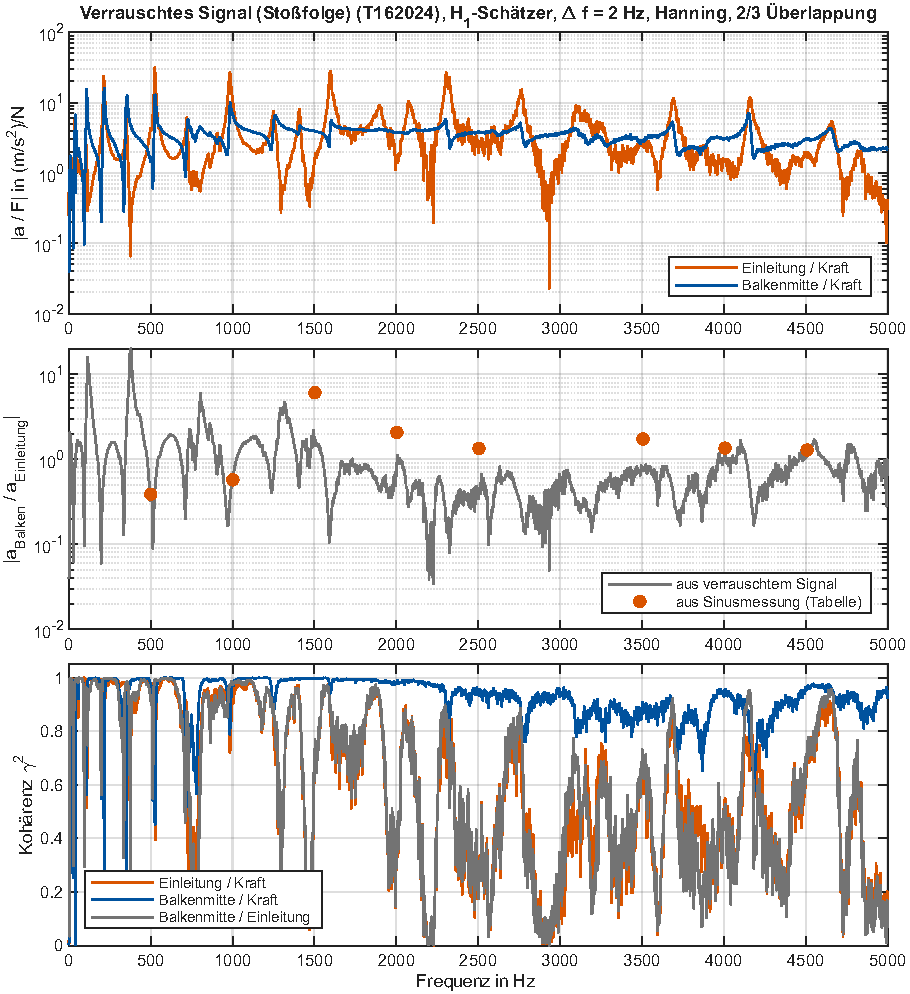
\includegraphics[width=\textwidth]{A5_uebertragung}
  \caption{Verrauschtes Signal (\texttt{T162024}), $H_1$-Schätzer,
  $\Delta f=\SI{2}{\hertz}$, Hanning, \SI{66.7}{\percent} Überlappung. Oben:
  Inertanz an beiden Positionen. Mitte: Übertragungsfunktion Einleitung
  $\rightarrow$ Mitte mit den Werten aus \tab{tab:positionen}. Unten:
  Kohärenz.}
  \label{fig:uebertragung}
\end{figure}

\begin{table}[H]
  \centering
  \caption{Maxima der Inertanz in der Balkenmitte mit Kohärenz
  $\gamma^2 \ge 0{,}8$ (Inertanzen in \si{(\metre\per\second\squared)\per\newton}).}
  \label{tab:resonanzen}
  \begin{tabular}{rrrr}
    \toprule
    $f$ in Hz & $|a_\text{Mitte}/F|$ & $|a_\text{Einl.}/F|$ & $\gamma^2_\text{Mitte}$ \\
    \midrule
    \tabinput{tab_resonanzen}
    \bottomrule
  \end{tabular}
\end{table}

\paragraph{Impulsanregung.} Aus den beiden Impulsmessungen (Versuch~3)
lassen sich die Inertanzen ebenfalls bestimmen (\abb{fig:impulsuebertragung},
ein Block von \SI{0.25}{\second} ab dem Impuls). Die Kurven zeigen dieselben
Tendenzen, sind aber stark verrauscht. Ursache ist die geringe Energie des
Impulses: Bei einer Spitzenkraft von nur \SI{0.75}{\newton} und einer Dauer
von \SI{0.04}{\milli\second} verteilt sich die Kraft auf einen
Frequenzbereich bis über \SI{10}{\kilo\hertz}, die Kraftdichte je Hertz ist
entsprechend klein. Ohne Mittelung über mehrere Impulse ist das
Signal-Rausch-Verhältnis zu gering; die Stoßfolge aus Versuch~4 liefert
dagegen durch die Mittelung über 184 Blöcke deutlich bessere Ergebnisse.

\begin{figure}[!htb]
  \centering
  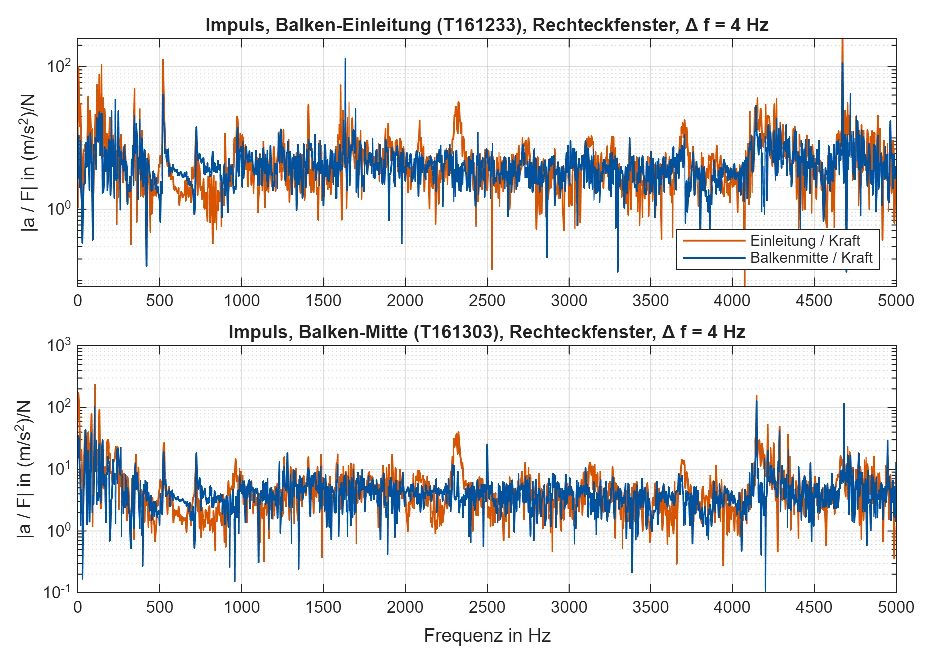
\includegraphics[width=\textwidth]{A5_impuls}
  \caption{Inertanz an beiden Positionen aus den Impulsmessungen
  \texttt{T161233} und \texttt{T161303} (Rechteckfenster, ein Block,
  $\Delta f=\SI{4}{\hertz}$).}
  \label{fig:impulsuebertragung}
\end{figure}

\paragraph{Fazit Sensorposition.} Das gemessene Spektrum ist immer das
Produkt aus Anregung und Übertragungsverhalten der Struktur zwischen
Anregungs- und Messort. Ein Sensor im Anregungspunkt sieht zudem
Antiresonanzen, in denen sich nur der Rest der Struktur bewegt. Je nach
Sensorposition werden Frequenzen um mehr als
\SI{20}{\decibel} verstärkt oder abgeschwächt (hier \SI{-8}{\decibel} bis
\SI{+16}{\decibel} allein für die Harmonischen der Sinusanregung); liegt der
Sensor in einem Schwingungsknoten, wird die zugehörige Eigenform nicht
erfasst. Messpunkte müssen daher bewusst gewählt werden (nicht in Knoten,
möglichst an Stellen großer Schwingungsamplitude), und Ergebnisse
verschiedener Messpunkte sind nur unter Angabe der Position vergleichbar.
Zur Ermittlung von Strukturresonanzen ist eine Übertragungsfunktion mit
gemessener Anregungskraft und ausreichender Mittelung vorzuziehen.

% ==================================================================
\section{Zusammenfassung}
% ==================================================================
Die Untersuchungen belegen, dass das Ergebnis einer Fourieranalyse nie
\glqq falsch\grqq, aber stets von den Daten und der Parametrierung abhängig
ist:
\begin{description}
  \item[Messdaten:] Vier der 19 Messungen waren nicht verwendbar (Testmessung,
    Messdauer kürzer als ein Block, zwei wiederholte Impulsmessungen). Sie
    wurden durch eine automatische Plausibilitätsprüfung erkannt und
    ausgeschlossen.
  \item[Abtastrate:] bestimmt den Frequenzbereich ($f_s/2$). Ohne
    AA-Filter erscheinen Harmonische bis \SI{5.5}{\kilo\hertz} mit voller
    Amplitude als scheinbare Linien unterhalb von \SI{1600}{\hertz}; das
    Messsystem filtert dies intern zuverlässig heraus. Bei Impulsen werden
    Spitzenwerte bei \SI{3.2}{\kilo\hertz} um bis zu \SI{77}{\percent}
    unterschätzt.
  \item[Fensterfunktion:] bestimmt Amplitudenfehler und Leckeffekt. Liegt die
    Signalfrequenz zwischen zwei Linien, betragen die Fehler
    \SI{36}{\percent} (Rechteck), \SI{15}{\percent} (Hanning) und
    \SI{0.2}{\percent} (Flattop).
  \item[Frequenzauflösung:] $T\cdot\Delta f = 1$. Feine Auflösung trennt
    benachbarte Frequenzen, erfordert aber lange Messungen, liefert wenige
    Mittelungen und eine schlechte Zeitauflösung; bei abklingenden
    Signalen erhöht sie das Rauschen.
  \item[Spektraldarstellung:] $\Sx$ gibt Sinusamplituden unabhängig von den
    Parametern wieder, $\Gxx$ breitbandige Signale. Nur $\Gxx$ erfüllt die
    Energiebilanz unabhängig vom Fenster.
  \item[Sensorposition:] Das Amplitudenverhältnis zwischen Einleitung und
    Balkenmitte schwankt zwischen \SI{-8}{\decibel} und \SI{+16}{\decibel};
    Resonanzen und Schwingungsknoten bestimmen, was ein Sensor
    \glqq sieht\grqq.
\end{description}
Für die Praxis folgt: Orientierungsmessung mit hoher Abtastrate,
Zeitsignal und Messdauer prüfen, Parameter ($f_s$, $\Delta f$, Fenster,
Überlappung, Darstellung) an Signal und Fragestellung anpassen und stets mit
dem Ergebnis dokumentieren -- nur bei gleicher Parametrierung sind Ergebnisse
vergleichbar.

% ==================================================================
\begin{thebibliography}{9}
  \bibitem{esefeld} Esefeld, B.: \emph{MTP/VTP Schwingungsanalyse},
    Versuchsunterlage, Hochschule München FK03, Labor für
    Schwingungstechnik und Maschinendynamik, 2026.
  \bibitem{kuttner} Kuttner, T.; Rohnen, A.: \emph{Praxis der
    Schwingungsmessung -- Messtechnik und Signalanalyse mit MATLAB},
    2.~Aufl., Springer Vieweg, Wiesbaden, 2019.
  \bibitem{zollner} Zollner, M.: \emph{Frequenzanalyse},
    Autoren-Selbstverlag, Regensburg, 1999.
  \bibitem{moeser} Möser, M. (Hrsg.): \emph{Messtechnik der Akustik},
    Springer-Verlag, Berlin, 2010.
  \bibitem{kammeyer} Kammeyer, K.\,D.: \emph{Digitale Signalverarbeitung},
    6.~Aufl., Teubner, 2006.
  \bibitem{din1311} DIN 1311:2000: \emph{Schwingungen und schwingungsfähige Systeme}.
  \bibitem{din45662} DIN 45662:1996-12: \emph{Schwingungsmesseinrichtung --
    Allgemeine Anforderungen und Begriffe}.
\end{thebibliography}

% ==================================================================
\appendix
\clearpage
\section{MATLAB-Quellcode}\label{sec:anhang}
% ==================================================================
Die komplette Auswertung wird mit \texttt{run\_alle.m} gestartet und erzeugt
alle Abbildungen und Tabellen dieses Berichts. Verwendet werden die
Funktionen der Signal Processing Toolbox (\texttt{hann}, \texttt{flattopwin},
\texttt{enbw}, \texttt{spectrogram}, \texttt{tfestimate}, \texttt{mscohere},
\texttt{resample}, \texttt{findpeaks}). Die Zuordnung der Messdateien und die
automatische Prüfung auf ungültige Messungen erfolgt in
\texttt{lib/messkatalog.m}.

\subsection*{Hauptskript und Hilfsfunktionen}
\lstinputlisting[title={run\_alle.m}]{../Auswertung_MATLAB/run_alle.m}
\lstinputlisting[title={lib/messkatalog.m}]{../Auswertung_MATLAB/lib/messkatalog.m}
\lstinputlisting[title={lib/lade\_messung.m}]{../Auswertung_MATLAB/lib/lade_messung.m}
\lstinputlisting[title={lib/spektrum.m}]{../Auswertung_MATLAB/lib/spektrum.m}
\lstinputlisting[title={lib/fenster.m}]{../Auswertung_MATLAB/lib/fenster.m}

\subsection*{Auswerteskripte}
\lstinputlisting[title={A0\_Zeitsignale.m}]{../Auswertung_MATLAB/A0_Zeitsignale.m}
\lstinputlisting[title={A1\_Abtastrate.m}]{../Auswertung_MATLAB/A1_Abtastrate.m}
\lstinputlisting[title={A2\_Fensterfunktion.m}]{../Auswertung_MATLAB/A2_Fensterfunktion.m}
\lstinputlisting[title={A3\_Frequenzaufloesung.m}]{../Auswertung_MATLAB/A3_Frequenzaufloesung.m}
\lstinputlisting[title={A4\_Spektraldarstellung.m}]{../Auswertung_MATLAB/A4_Spektraldarstellung.m}
\lstinputlisting[title={A5\_Sensorposition.m}]{../Auswertung_MATLAB/A5_Sensorposition.m}

\end{document}
